\documentclass[10pt]{beamer}
\usetheme{metropolis}

% ── Packages ──
\usepackage{amsmath,amssymb,amsthm}
\usepackage{tikz}
\usetikzlibrary{positioning,arrows.meta,fit,matrix,backgrounds,calc,shapes.geometric}
\usepackage{graphicx}
\usepackage{array}
\usepackage{etoolbox}

% ── Theorem environments ──
\theoremstyle{definition}
\newtheorem{defi}{Definition}[section]
\newtheorem{prop}{Proposition}[section]
\newtheorem{thm}{Theorem}[section]
\newtheorem{cor}{Corollary}[section]

% Custom theorem styles with colors
\setbeamercolor{block title}{bg=red!75!black,fg=white}
\setbeamercolor{block body}{bg=yellow!10!white}

% Proposition uses yellow title
\AtBeginEnvironment{prop}{%
  \setbeamercolor{block title}{bg=yellow!75!black,fg=black}%
  \setbeamercolor{block body}{bg=yellow!10!white}%
}
\AtEndEnvironment{prop}{%
  \setbeamercolor{block title}{bg=red!75!black,fg=white}%
}

% Theorem uses yellow title
\AtBeginEnvironment{thm}{%
  \setbeamercolor{block title}{bg=yellow!75!black,fg=black}%
  \setbeamercolor{block body}{bg=yellow!10!white}%
}
\AtEndEnvironment{thm}{%
  \setbeamercolor{block title}{bg=red!75!black,fg=white}%
}

% ── Highlighting ──
\newcommand{\x}[1]{\alert{\textbf{#1}}}

\title{Lecture 7: Linear Transformation and Projection}
\subtitle{MATH203 Applied Linear Algebra}
\date{}

\begin{document}
\maketitle

% ═══════════════════════════════════════
% §0 MOTIVATION
% ═══════════════════════════════════════
\section{From Static to Dynamic}

\begin{frame}{Recap: What We Know So Far}

In Lectures 1--6, matrices were \x{static objects}:

\vspace{0.5em}

\begin{itemize}
\item Ingredient tables (recipes for making products)
\item Containers of column vectors and row vectors
\item Objects with four fundamental subspaces
\end{itemize}

\vspace{1em}

\x{Today}: Matrices become \x{dynamic} --- they \x{act} on vectors.

\vspace{1em}

$$\mathbf{v} \xrightarrow{\quad A \quad} A\mathbf{v}$$

\end{frame}

\begin{frame}{Roadmap for Today}

\x{Part 1}: Linear Transformations
\begin{itemize}
\item What does ``preserving linear structure'' mean?
\end{itemize}

\vspace{0.5em}

\x{Part 2}: Projection Operators ($P^2 = P$)
\begin{itemize}
\item The sunlight-and-floor model
\end{itemize}

\vspace{0.5em}

\x{Part 3}: Basic Properties of Projections
\begin{itemize}
\item Interchanging property, disjoint property
\end{itemize}

\vspace{0.5em}

\x{Part 4}: Orthogonal Projections ($P = P^T$)
\begin{itemize}
\item When sunlight is perpendicular to the floor
\end{itemize}

\end{frame}

% ═══════════════════════════════════════
% §1 LINEAR TRANSFORMATIONS
% ═══════════════════════════════════════
\section{Linear Transformations}

\begin{frame}{Definition}

\begin{defi}[Linear Transformation]
A function $T: V \to W$ between vector spaces is a \x{linear transformation} if
$$T(\lambda \mathbf{v} + \mathbf{w}) = \lambda\, T(\mathbf{v}) + T(\mathbf{w})$$
for all $\mathbf{v}, \mathbf{w} \in V$ and all scalars $\lambda$.
\end{defi}

\vspace{1em}

Equivalently, two properties:
\begin{enumerate}
\item \x{Additivity}: $T(\mathbf{v} + \mathbf{w}) = T(\mathbf{v}) + T(\mathbf{w})$
\item \x{Homogeneity}: $T(\lambda \mathbf{v}) = \lambda\, T(\mathbf{v})$
\end{enumerate}

\end{frame}

\begin{frame}{Geometric Meaning}

Linear transformations \x{preserve linear structure}:

\vspace{1em}

\begin{center}
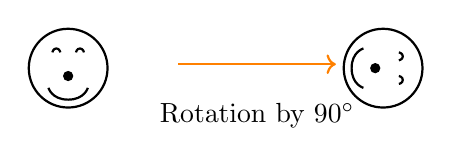
\begin{tikzpicture}[scale=0.5]
% Rotation
\draw[thick] (0cm,0cm) circle(1cm);
\draw[thick] plot [smooth,tension=1.5] coordinates{(-0.5,-0.5) (0,-0.8) (0.5,-0.5)};
\draw [thick, fill=black] (0,-0.2) circle (0.1);
\draw[thick] plot [smooth,tension=1.5] coordinates{(-0.4,0.4) (-0.3,0.5) (-0.2,0.4)};
\draw[thick] plot [smooth,tension=1.5] coordinates{(0.4,0.4) (0.3,0.5) (0.2,0.4)};
\draw[thick] (8cm,0cm) circle(1cm);
\draw[thick] plot [smooth,tension=1.5] coordinates{(7.5,0.5) (7.2,0) (7.5,-0.5)};
\draw [thick, fill=black] (7.8,0) circle (0.1);
\draw[thick] plot [smooth,tension=1.5] coordinates{(8.4,0.4) (8.5,0.3) (8.4,0.2)};
\draw[thick] plot [smooth,tension=1.5] coordinates{(8.4,-0.4) (8.5,-0.3) (8.4,-0.2)};
\draw[thick,->,orange](2.8,0.1)--(6.8,0.1);
\node at (4.8, -1.2) {Rotation by $90^\circ$};
\end{tikzpicture}
\end{center}

\vspace{0.3cm}

\begin{center}

\begin{tikzpicture}[scale=0.5]
% Reflection
\draw[thick] (0cm,0cm) circle(1cm);
\draw[thick] plot [smooth,tension=1.5] coordinates{(-0.5,-0.5) (0,-0.8) (0.5,-0.5)};
\draw [thick, fill=black] (0,-0.2) circle (0.1);
\draw[thick] plot [smooth,tension=1.5] coordinates{(-0.4,0.4) (-0.3,0.5) (-0.2,0.4)};
\draw[thick] plot [smooth,tension=1.5] coordinates{(0.4,0.4) (0.3,0.5) (0.2,0.4)};
\draw[thick] (8cm,0cm) circle(1cm);
\draw[thick] plot [smooth,tension=1.5] coordinates{(7.5,0.5) (8,0.8) (8.5,0.5)};
\draw [thick, fill=black] (8,0.2) circle (0.1);
\draw[thick] plot [smooth,tension=1.5] coordinates{(7.6,-0.4) (7.7,-0.5) (7.8,-0.4)};
\draw[thick] plot [smooth,tension=1.5] coordinates{(8.4,-0.4) (8.3,-0.5) (8.2,-0.4)};
\draw[thick,->,orange](2.8,0.1)--(6.8,0.1);
\node at (4.8, -1.2) {Reflection};
\end{tikzpicture}
\end{center}

\vspace{0.3cm}

\begin{center}
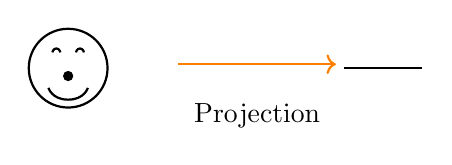
\begin{tikzpicture}[scale=0.5]
% Projection
\draw[thick] (0cm,0cm) circle(1cm);
\draw[thick] plot [smooth,tension=1.5] coordinates{(-0.5,-0.5) (0,-0.8) (0.5,-0.5)};
\draw [thick, fill=black] (0,-0.2) circle (0.1);
\draw[thick] plot [smooth,tension=1.5] coordinates{(-0.4,0.4) (-0.3,0.5) (-0.2,0.4)};
\draw[thick] plot [smooth,tension=1.5] coordinates{(0.4,0.4) (0.3,0.5) (0.2,0.4)};
\draw[thick] (7,0)--(9,0);
\draw[thick,->,orange](2.8,0.1)--(6.8,0.1);
\node at (4.8, -1.2) {Projection};
\end{tikzpicture}
\end{center}

\end{frame}

\begin{frame}{Common Examples in $\mathbb{R}^2$}

\begin{enumerate}
\item \x{Rotation by $90^\circ$}:
$T\begin{pmatrix} x \\ y \end{pmatrix} = \begin{pmatrix} -y \\ x \end{pmatrix}$
\quad $A = \begin{pmatrix} 0 & -1 \\ 1 & 0 \end{pmatrix}$

\vspace{0.5em}

\item \x{Reflection across $x$-axis}:
$T\begin{pmatrix} x \\ y \end{pmatrix} = \begin{pmatrix} x \\ -y \end{pmatrix}$
\quad $A = \begin{pmatrix} 1 & 0 \\ 0 & -1 \end{pmatrix}$

\vspace{0.5em}

\item \x{Scaling by 2}:
$T\begin{pmatrix} x \\ y \end{pmatrix} = \begin{pmatrix} 2x \\ 2y \end{pmatrix}$
\quad $A = \begin{pmatrix} 2 & 0 \\ 0 & 2 \end{pmatrix}$

\vspace{0.5em}

\item \x{Projection onto $x$-axis}:
$T\begin{pmatrix} x \\ y \end{pmatrix} = \begin{pmatrix} x \\ 0 \end{pmatrix}$
\quad $A = \begin{pmatrix} 1 & 0 \\ 0 & 0 \end{pmatrix}$
\end{enumerate}

\end{frame}

\begin{frame}{Matrix Representation}

\begin{prop}[Matrix Representation]
Every linear transformation $T: \mathbb{R}^n \to \mathbb{R}^m$ can be written as
$$T(\mathbf{v}) = A\mathbf{v}$$
for some $m \times n$ matrix $A$.

Conversely, every matrix defines a linear transformation.
\end{prop}

\vspace{1em}

\begin{defi}[Linear Operator]
When the domain and codomain are the same ($T: V \to V$), we call $T$ a \x{linear operator}.

Represented by \x{square matrices}.
\end{defi}

\vspace{1em}

For the rest of this lecture, we focus on \x{linear operators} (square matrices).

\end{frame}

% ═══════════════════════════════════════
% §2 PROJECTION OPERATORS
% ═══════════════════════════════════════
\section{Projection Operators}

\begin{frame}{Definition}

\begin{defi}[Projection Operator (Idempotent)]
A matrix $P$ is called a \x{projection operator} if
$$P^2 = P$$
\end{defi}

\vspace{1em}

The name ``idempotent'' comes from Latin:

\begin{center}
\textit{idem} (same) + \textit{potent} (power)
\end{center}

\vspace{0.5em}

Applying the operation multiple times gives the \x{same result} as applying it once.

\end{frame}

\begin{frame}{The Sunlight-and-Floor Model}

\begin{center}
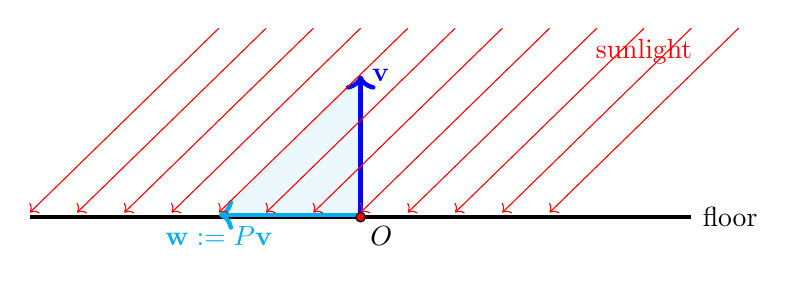
\begin{tikzpicture}[scale=0.6]
\draw[ultra thick](-7,0)--(7,0) node[right]{floor};
\draw[ultra thick,->,blue](0,0)--(0,3) node[right]{$\mathbf{v}$};
\draw[opacity=0.08,fill=cyan] (0,0)--(0,3)--(-3,0);
\draw[ultra thick,->,cyan](0,0.05)--(-3,0.05) node[below]{$\mathbf{w}:=P\mathbf{v}$};
\foreach\x in {-3,...,8}{
	\draw [red,->](\x,4)--(-4+\x,0.1);
}
\draw[fill=red] (0,0) circle[radius=0.1] node[below right]{$O$};
\node[red] at (6,3.5) {sunlight};
\end{tikzpicture}
\end{center}

\vspace{0.5em}

\begin{itemize}
\item A \x{vector $\mathbf{v}$} stands at the origin (like a tree)
\item \x{Sunlight} shines from some direction
\item The projection $P$ maps $\mathbf{v}$ to its \x{shadow} $\mathbf{w} = P\mathbf{v}$ on the floor
\end{itemize}

\vspace{0.5em}

The sunlight direction \x{need not} be perpendicular to the floor!

\end{frame}

\begin{frame}{Why $P^2 = P$?}

We require $P^2 = P$. This means $P^2\mathbf{v} = P\mathbf{v}$ for any $\mathbf{v}$.

\vspace{1em}

\x{Geometrically}: \textbf{The shadow of a shadow is the shadow itself.}

\vspace{1em}

\begin{center}
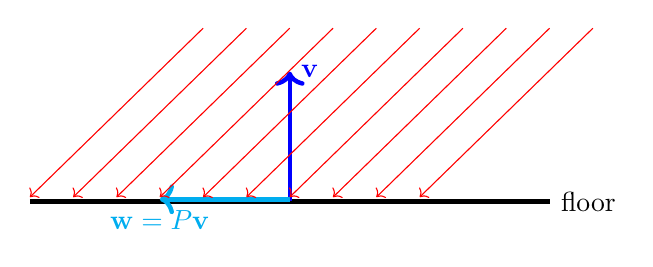
\begin{tikzpicture}[scale=0.55]
\draw[ultra thick](-6,0)--(6,0) node[right]{floor};
\draw[ultra thick,->,blue](0,0)--(0,3) node[right]{$\mathbf{v}$};
\draw[ultra thick,->,cyan](0,0.05)--(-3,0.05) node[below]{$\mathbf{w} = P\mathbf{v}$};
\foreach\x in {-2,...,7}{
	\draw [red,->](\x,4)--(-4+\x,0.1);
}
\end{tikzpicture}
\end{center}

\vspace{0.5em}

Since $\mathbf{w} = P\mathbf{v}$ lies on the floor, the shadow of $\mathbf{w}$ is \x{itself}:
$$P\mathbf{w} = \mathbf{w} \quad\implies\quad P(P\mathbf{v}) = P\mathbf{v} \quad\implies\quad P^2 = P$$

\end{frame}

\begin{frame}{Three Key Questions}

We defined projection only by $P^2 = P$. But intuitively a projection needs:

\vspace{1em}

\begin{enumerate}
\item If $P^2 = P$, how do we define \x{the floor}?

\vspace{0.5em}

\item If $P^2 = P$, how do we define \x{the direction of sunlight}?

\vspace{0.5em}

\item After specifying these, why is $P\mathbf{v}$ exactly \x{the shadow} of $\mathbf{v}$?
\end{enumerate}

\vspace{1em}

Let us answer them one by one.

\end{frame}

\begin{frame}{Question 1: Vectors Pointing Toward the Sun}

If a vector $\mathbf{v}$ points \x{toward the sun}, what is its shadow?

\begin{center}
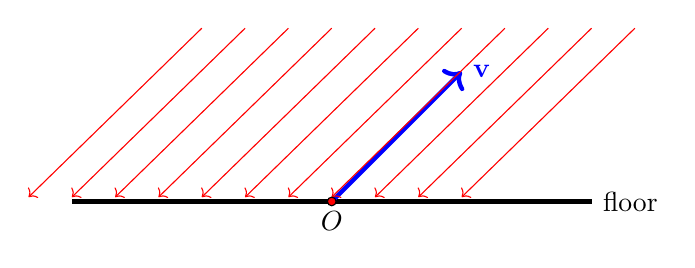
\begin{tikzpicture}[scale=0.55]
\draw[ultra thick](-6,0)--(6,0) node[right]{floor};
\draw[ultra thick,->,blue](0,0)--(3,3) node[right]{$\mathbf{v}$};
\foreach\x in {-3,...,7}{
	\draw [red,->](\x,4)--(-4+\x,0.1);
}
\draw[fill=red] (0,0) circle[radius=0.1] node[below]{$O$};
\end{tikzpicture}
\end{center}

\vspace{0.5em}

\x{Answer}: $P\mathbf{v} = \mathbf{0}$ (no shadow!)

\vspace{0.5em}

The set of all such vectors:
$$\{\mathbf{v} \in V : P\mathbf{v} = \mathbf{0}\} = \operatorname{Null}(P)$$

\vspace{0.5em}

$\operatorname{Null}(P)$ describes the \x{direction of sunlight}.

\end{frame}

\begin{frame}{Question 2: Vectors Lying on the Floor}

If a vector $\mathbf{w}$ lies \x{on the floor}, what is its shadow?

\begin{center}
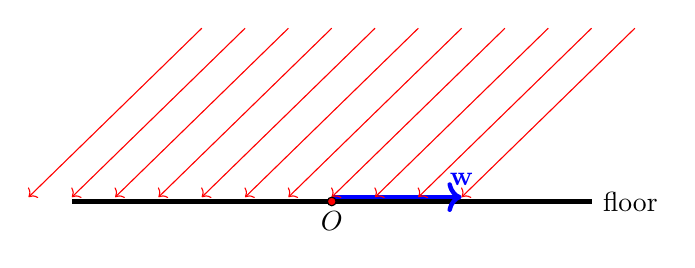
\begin{tikzpicture}[scale=0.55]
\draw[ultra thick](-6,0)--(6,0) node[right]{floor};
\draw[ultra thick,->,blue](0,0.1)--(3,0.1) node[above]{$\mathbf{w}$};
\foreach\x in {-3,...,7}{
	\draw [red,->](\x,4)--(-4+\x,0.1);
}
\draw[fill=red] (0,0) circle[radius=0.1] node[below]{$O$};
\end{tikzpicture}
\end{center}

\vspace{0.5em}

\x{Answer}: $P\mathbf{w} = \mathbf{w}$ (a vector on the floor is its own shadow)

\vspace{0.5em}

Two equivalent descriptions of the floor:
$$\underbrace{\{\mathbf{w} : \mathbf{w} = P\mathbf{v} \text{ for some } \mathbf{v}\}}_{\operatorname{Col}(P)} \;=\; \underbrace{\{\mathbf{w} : P\mathbf{w} = \mathbf{w}\}}_{\text{fixed points of } P}$$

\vspace{0.5em}

$\operatorname{Col}(P)$ describes \x{the floor}.

\end{frame}

\begin{frame}{Question 3: Why Is $P\mathbf{v}$ the Shadow?}

Given $P^2 = P$, with the floor $\operatorname{Col}(P)$ and sunlight $\operatorname{Null}(P)$:

\begin{center}
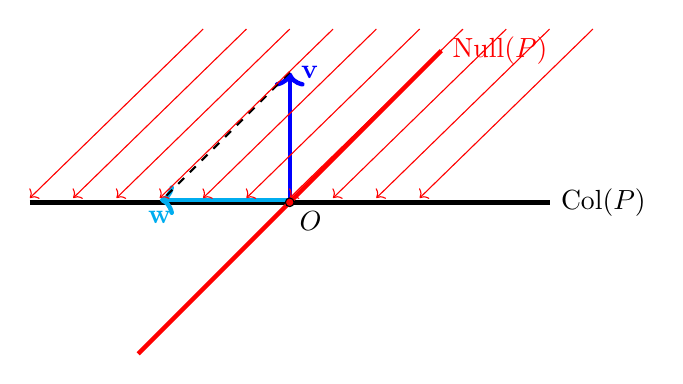
\begin{tikzpicture}[scale=0.55]
\draw[ultra thick](-6,0)--(6,0) node[right]{$\operatorname{Col}(P)$};
\draw[ultra thick,red](-3.5,-3.5)--(3.5,3.5) node[right]{$\operatorname{Null}(P)$};
\draw[ultra thick,->,blue](0,0)--(0,3) node[right]{$\mathbf{v}$};
\draw[ultra thick,->,cyan](0,0.05)--(-3,0.05) node[below]{$\mathbf{w}$};
\draw[dashed,thick] (0,3)--(-3,0);
\foreach\x in {-2,...,7}{
	\draw [red,->](\x,4)--(-4+\x,0.1);
}
\draw[fill=red] (0,0) circle[radius=0.1] node[below right]{$O$};
\end{tikzpicture}
\end{center}

\vspace{0.3em}

The shadow $\mathbf{w}$ must satisfy:
\begin{enumerate}
\item $\mathbf{w} \in \operatorname{Col}(P)$ \quad (shadow lies on the floor)
\item $\mathbf{v} - \mathbf{w} \in \operatorname{Null}(P)$ \quad (line from $\mathbf{v}$ to $\mathbf{w}$ follows sunlight)
\end{enumerate}

\end{frame}

\begin{frame}{The Proof}

\begin{prop}[Projection gives the shadow]
If $P^2 = P$ and $\mathbf{w}$ is the geometric shadow (i.e.\ $\mathbf{w} \in \operatorname{Col}(P)$ and $\mathbf{v} - \mathbf{w} \in \operatorname{Null}(P)$), then $\mathbf{w} = P\mathbf{v}$.
\end{prop}

\textbf{Proof}:

Since $\mathbf{w} \in \operatorname{Col}(P)$, we have $\mathbf{w} = P\mathbf{x}$ for some $\mathbf{x}$.
$$P\mathbf{w} = P(P\mathbf{x}) = P^2\mathbf{x} = P\mathbf{x} = \mathbf{w}$$

Since $\mathbf{v} - \mathbf{w} \in \operatorname{Null}(P)$:
$$P(\mathbf{v} - \mathbf{w}) = \mathbf{0} \quad\implies\quad P\mathbf{v} = P\mathbf{w}$$

Combining:
$$P\mathbf{v} = P\mathbf{w} = \mathbf{w} \qquad \qed$$

\end{frame}

\begin{frame}{Summary: The Sunlight Model}

\begin{alertblock}{Projection Operator Summary}
As long as $P^2 = P$, the operator $P$ is a projection:

\begin{enumerate}
\item For any $\mathbf{v} \in V$:
\begin{itemize}
\item $P\mathbf{v}$ = the shadow
\item $(I - P)\mathbf{v} = \mathbf{v} - P\mathbf{v}$ = vector pointing toward the sun
\end{itemize}

\vspace{0.3em}

\item $\operatorname{Null}(P)$ = \x{direction of sunlight}

\vspace{0.3em}

\item $\operatorname{Col}(P)$ = \x{the floor}
\begin{itemize}
\item For any $\mathbf{w} \in \operatorname{Col}(P)$: $P\mathbf{w} = \mathbf{w}$
\end{itemize}
\end{enumerate}
\end{alertblock}

\end{frame}

% ═══════════════════════════════════════
% §3 BASIC PROPERTIES
% ═══════════════════════════════════════
\section{Basic Properties of Projections}

\begin{frame}{Column Space Membership Test}

\begin{prop}[Floor Membership Test]
Let $P$ be a projection. For any $\mathbf{y} \in \mathbb{R}^n$:
$$\mathbf{y} \in \operatorname{Col}(P) \quad\iff\quad P\mathbf{y} = \mathbf{y}$$
\end{prop}

\textbf{Proof}:

($\Rightarrow$): If $\mathbf{y} \in \operatorname{Col}(P)$, then $\mathbf{y} = P\mathbf{x}$ for some $\mathbf{x}$.
$$P\mathbf{y} = P(P\mathbf{x}) = P^2\mathbf{x} = P\mathbf{x} = \mathbf{y} \quad\checkmark$$

($\Leftarrow$): If $P\mathbf{y} = \mathbf{y}$, then $\mathbf{y} \in \operatorname{Col}(P)$ by definition. $\quad\checkmark$

\vspace{1em}

\x{Geometric meaning}: A vector is on the floor $\iff$ it equals its own shadow.

\end{frame}

\begin{frame}{Exercise: Testing Membership}

\begin{exampleblock}{Exercise}
The following matrix is a projection:
$$P = \begin{pmatrix} 0 & 0 & 0 \\ -1 & 1 & 0 \\ -1 & 0 & 1 \end{pmatrix}$$

Calculate $P\begin{pmatrix} 0 \\ 2 \\ 0 \end{pmatrix}$. Is $\begin{pmatrix} 0 \\ 2 \\ 0 \end{pmatrix} \in \operatorname{Col}(P)$?
\end{exampleblock}

\vspace{1em}

\textit{Hint}: Use the membership test --- check whether $P\mathbf{y} = \mathbf{y}$.

\end{frame}

\begin{frame}{The Companion Projection: $I - P$}

\begin{prop}[$I - P$ is also a Projection]
If $P^2 = P$, then $I - P$ is also a projection.
\end{prop}

\textbf{Proof}:
$$(I - P)^2 = I - 2P + P^2 = I - 2P + P = I - P \quad\checkmark$$

\vspace{1em}

\x{Geometric interpretation}:

\begin{center}
\begin{tabular}{ll}
$P$ & projects \x{onto the floor} \\
$I - P$ & projects \x{in the direction of sunlight} \\
\end{tabular}
\end{center}

\vspace{0.5em}

For any $\mathbf{v}$:
$$\underbrace{P\mathbf{v}}_{\text{shadow on floor}} + \underbrace{(I-P)\mathbf{v}}_{\text{displacement toward sun}} = \mathbf{v}$$

\end{frame}

\begin{frame}{The Interchanging Property}

\begin{prop}[Column Space and Null Space Interchange]
For any projection $P$:
$$\operatorname{Col}(P) = \operatorname{Null}(I - P)$$
$$\operatorname{Col}(I - P) = \operatorname{Null}(P)$$
\end{prop}

\textbf{Proof} (first equality):

($\subseteq$): $\mathbf{v} \in \operatorname{Col}(P) \implies P\mathbf{v} = \mathbf{v} \implies (I-P)\mathbf{v} = \mathbf{0} \implies \mathbf{v} \in \operatorname{Null}(I-P)$

\vspace{0.3em}

($\supseteq$): $\mathbf{v} \in \operatorname{Null}(I-P) \implies (I-P)\mathbf{v} = \mathbf{0} \implies \mathbf{v} = P\mathbf{v} \implies \mathbf{v} \in \operatorname{Col}(P)$

\vspace{1em}

\begin{center}
\begin{tabular}{c|c}
\textbf{For $P$} & \textbf{For $I - P$} \\
\hline
$\operatorname{Col}(P)$ & $= \operatorname{Null}(I - P)$ \\
$\operatorname{Null}(P)$ & $= \operatorname{Col}(I - P)$ \\
\end{tabular}
\end{center}

\x{Beautiful!} $P$ and $I - P$ \x{interchange} their column spaces and null spaces.

\end{frame}

\begin{frame}{The Disjoint Property}

\begin{prop}[Column Space and Null Space Are Disjoint]
For any projection $P$:
$$\operatorname{Col}(P) \cap \operatorname{Null}(P) = \{\mathbf{0}\}$$
\end{prop}

\textbf{Proof}:

Let $\mathbf{v} \in \operatorname{Col}(P) \cap \operatorname{Null}(P)$.

\vspace{0.3em}

$\mathbf{v} \in \operatorname{Col}(P) \implies P\mathbf{v} = \mathbf{v}$

$\mathbf{v} \in \operatorname{Null}(P) \implies P\mathbf{v} = \mathbf{0}$

\vspace{0.3em}

Therefore $\mathbf{v} = \mathbf{0}$. \qed

\vspace{1em}

\x{Geometric meaning}: The floor and the sunlight direction \x{only meet at the origin}.

\vspace{0.5em}

A non-zero vector cannot simultaneously be on the floor and point toward the sun.

\end{frame}

% ═══════════════════════════════════════
% §4 ORTHOGONAL PROJECTIONS
% ═══════════════════════════════════════
\section{Orthogonal Projections}

\begin{frame}{Motivation: Perpendicular Sunlight}

In Lecture 6, we discovered:
$$\operatorname{Col}(A^T) \perp \operatorname{Null}(A)$$

\vspace{1em}

A natural question in the sunlight-floor model:

\vspace{0.5em}

\begin{center}
\x{Can the sunlight shine perpendicular to the floor?}
\end{center}

\vspace{1em}

That is: can we have $\operatorname{Col}(P) \perp \operatorname{Null}(P)$?

\end{frame}

\begin{frame}{Definition}

\begin{defi}[Orthogonal Projection]
A projection $P$ ($P^2 = P$) is called an \x{orthogonal projection} if
$$\operatorname{Col}(P) \perp \operatorname{Null}(P)$$
That is, $\mathbf{v}^T\mathbf{w} = 0$ for every $\mathbf{v} \in \operatorname{Col}(P)$ and $\mathbf{w} \in \operatorname{Null}(P)$.
\end{defi}

\vspace{1em}

In the sunlight model: the sunlight shines \x{perpendicular} to the floor.

\end{frame}

\begin{frame}{Example: Orthogonal vs Oblique}

Two projections onto the \x{same floor} $W = \operatorname{span}\left\{\begin{pmatrix} 1 \\ 1 \end{pmatrix}\right\}$:

\vspace{0.5em}

\begin{columns}[T]
\begin{column}{0.48\textwidth}
\x{Orthogonal}: $P_1 = \frac{1}{2}\begin{pmatrix} 1 & 1 \\ 1 & 1 \end{pmatrix}$

\vspace{0.3em}

\begin{center}
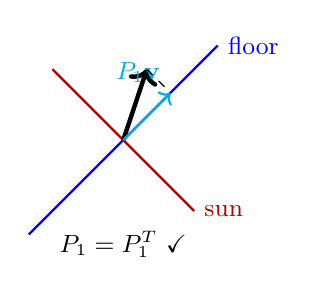
\begin{tikzpicture}[scale=0.6]
\draw[thick,blue](-2,-2)--(2,2) node[right]{\small floor};
\draw[thick,red!70!black](-1.5,1.5)--(1.5,-1.5) node[right]{\small sun};
\draw[->,ultra thick](0,0)--(0.5,1.5);
\draw[->,cyan,thick](0,0)--(1,1) node[above left]{\small $P_1\mathbf{v}$};
\draw[dashed](0.5,1.5)--(1,1);
\node at (0,-2.2) {\small $P_1 = P_1^T$ \checkmark};
\end{tikzpicture}
\end{center}
\end{column}

\begin{column}{0.48\textwidth}
\x{Oblique}: $P_2 = \begin{pmatrix} 1 & 0 \\ 1 & 0 \end{pmatrix}$

\vspace{0.3em}

\begin{center}
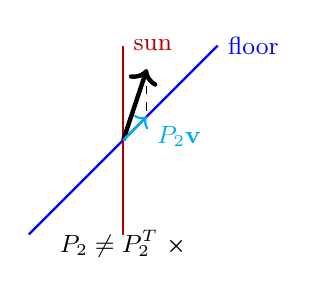
\begin{tikzpicture}[scale=0.6]
\draw[thick,blue](-2,-2)--(2,2) node[right]{\small floor};
\draw[thick,red!70!black](0,-2)--(0,2) node[right]{\small sun};
\draw[->,ultra thick](0,0)--(0.5,1.5);
\draw[->,cyan,thick](0,0)--(0.5,0.5) node[below right]{\small $P_2\mathbf{v}$};
\draw[dashed](0.5,1.5)--(0.5,0.5);
\node at (0,-2.2) {\small $P_2 \neq P_2^T$ \text{\texttimes}};
\end{tikzpicture}
\end{center}
\end{column}
\end{columns}

\vspace{0.5em}

Same floor, different sunlight. Only $P_1$ has \x{perpendicular sunlight}.

\end{frame}

\begin{frame}{Verification of the Example}

\x{Orthogonal} $P_1 = \frac{1}{2}\begin{pmatrix} 1 & 1 \\ 1 & 1 \end{pmatrix}$:

\begin{itemize}
\item $\operatorname{Col}(P_1) = \operatorname{span}\left\{\begin{pmatrix} 1 \\ 1 \end{pmatrix}\right\}$, \quad $\operatorname{Null}(P_1) = \operatorname{span}\left\{\begin{pmatrix} 1 \\ -1 \end{pmatrix}\right\}$
\item $\begin{pmatrix} 1 \\ 1 \end{pmatrix}^T \begin{pmatrix} 1 \\ -1 \end{pmatrix} = 1 - 1 = 0$ \checkmark \quad \x{Perpendicular!}
\item $P_1 = P_1^T$ \checkmark
\end{itemize}

\vspace{1em}

\x{Oblique} $P_2 = \begin{pmatrix} 1 & 0 \\ 1 & 0 \end{pmatrix}$:

\begin{itemize}
\item $\operatorname{Col}(P_2) = \operatorname{span}\left\{\begin{pmatrix} 1 \\ 1 \end{pmatrix}\right\}$, \quad $\operatorname{Null}(P_2) = \operatorname{span}\left\{\begin{pmatrix} 0 \\ 1 \end{pmatrix}\right\}$
\item $\begin{pmatrix} 1 \\ 1 \end{pmatrix}^T \begin{pmatrix} 0 \\ 1 \end{pmatrix} = 0 + 1 = 1 \neq 0$ \texttimes \quad \x{Not perpendicular!}
\item $P_2 \neq P_2^T$ \texttimes
\end{itemize}

\end{frame}

\begin{frame}{The Characterization Theorem}

\begin{thm}[Orthogonal Projection $\Leftrightarrow$ Symmetry]
Let $P$ be a projection ($P^2 = P$). The following are equivalent:
\begin{enumerate}
\item \textbf{Geometric}: $\operatorname{Col}(P) \perp \operatorname{Null}(P)$
\item \textbf{Algebraic}: $P = P^T$
\end{enumerate}
\end{thm}

\vspace{1em}

\x{Why this is powerful}: To check orthogonality, just compare entries: $p_{ij} = p_{ji}$.

\vspace{0.5em}

No need to compute column spaces, null spaces, or inner products!

\end{frame}

\begin{frame}{Proof: ($P = P^T$) $\Rightarrow$ ($\operatorname{Col}(P) \perp \operatorname{Null}(P)$)}

Assume $P = P^T$. Take $\mathbf{v} \in \operatorname{Col}(P)$ and $\mathbf{w} \in \operatorname{Null}(P)$.

\vspace{0.5em}

By Lecture 6: $\operatorname{Col}(A^T) \perp \operatorname{Null}(A)$ always holds.

\vspace{0.5em}

Since $P^T = P$:
$$\operatorname{Col}(P) = \operatorname{Col}(P^T) \perp \operatorname{Null}(P) \quad\checkmark$$

\vspace{1em}

\x{Alternative direct proof}: Since $P\mathbf{v} = \mathbf{v}$:

$$\mathbf{v}^T\mathbf{w} = (P\mathbf{v})^T\mathbf{w} = \mathbf{v}^T \underbrace{P^T}_{= P}\mathbf{w} = \mathbf{v}^T \underbrace{P\mathbf{w}}_{= \mathbf{0}} = 0 \quad\checkmark$$

\end{frame}

\begin{frame}{Proof: ($\operatorname{Col}(P) \perp \operatorname{Null}(P)$) $\Rightarrow$ ($P = P^T$)}

Assume $\operatorname{Col}(P) \perp \operatorname{Null}(P)$.

\vspace{0.5em}

For any $\mathbf{e}_i, \mathbf{e}_j$ (standard basis vectors):

\begin{itemize}
\item $P\mathbf{e}_i \in \operatorname{Col}(P)$
\item $(I - P)\mathbf{e}_j \in \operatorname{Null}(P)$ \quad (by interchanging property)
\end{itemize}

\vspace{0.5em}

By orthogonality assumption:
$$(P\mathbf{e}_i)^T(I - P)\mathbf{e}_j = 0 \quad \text{for all } i, j$$

\vspace{0.5em}

This is the $(i,j)$-entry of $P^T(I - P) = 0$, so:
$$P^T = P^T P$$

\vspace{0.5em}

Taking transpose:
$$P = (P^TP)^T = P^TP = P^T \quad\qed$$

\end{frame}

\begin{frame}{Orthogonal Projection: Summary}

\begin{alertblock}{Orthogonal Projection = Two Algebraic Conditions}
$$\boxed{P^2 = P \quad\text{and}\quad P = P^T}$$

The geometry of ``sunlight perpendicular to floor'' is captured by \x{matrix symmetry}.
\end{alertblock}

\vspace{1em}

\begin{exampleblock}{Exercise}
Fill in the blanks so that the following matrix is a projection:
$$P = \begin{pmatrix} 0.5 & \square \\ 0.5 & \square \end{pmatrix}$$
Is your answer an orthogonal projection?
\end{exampleblock}

\end{frame}

% ═══════════════════════════════════════
% §5 SUMMARY AND PREVIEW
% ═══════════════════════════════════════
\section{Summary}

\begin{frame}{What We Learned Today}

\x{1.\ Linear Transformation}: $T(\lambda \mathbf{v} + \mathbf{w}) = \lambda T(\mathbf{v}) + T(\mathbf{w})$
\begin{itemize}
\item Represented by matrices: $T(\mathbf{v}) = A\mathbf{v}$
\end{itemize}

\vspace{0.5em}

\x{2.\ Projection Operator}: $P^2 = P$
\begin{itemize}
\item $\operatorname{Col}(P)$ = floor, \quad $\operatorname{Null}(P)$ = sunlight
\end{itemize}

\vspace{0.5em}

\x{3.\ Basic Properties}:
\begin{itemize}
\item $\mathbf{y} \in \operatorname{Col}(P) \iff P\mathbf{y} = \mathbf{y}$
\item $I - P$ is also a projection
\item $\operatorname{Col}(P) = \operatorname{Null}(I - P)$ (interchanging)
\item $\operatorname{Col}(P) \cap \operatorname{Null}(P) = \{\mathbf{0}\}$ (disjoint)
\end{itemize}

\vspace{0.5em}

\x{4.\ Orthogonal Projection}: $P^2 = P$ and $P = P^T$
\begin{itemize}
\item Perpendicular sunlight $\iff$ symmetry
\end{itemize}

\end{frame}

\begin{frame}{Preview: Lecture 8}

\x{Lecture 8}: Cross-Filling Projections

\vspace{1em}

What happens when we \x{cross-fill} a projection matrix $P$?

\vspace{0.5em}

Something remarkable: each rank-one piece is \x{automatically a projection}!

\vspace{1em}

This will lead to:

\begin{itemize}
\item $\operatorname{rank}(P) = \operatorname{trace}(P)$ --- true \x{only} for projections
\item If $UV = I$, the factors must be \x{square and invertible}
\item Full-rank square matrices are always invertible
\end{itemize}

\end{frame}

\end{document}
